\section{Kinematic fit}
\label{sec:kineFit}
% ---- ---- ---- ---- ---- ---- ---- ---- ---- ---- ---- ---- ---- ---- ---- ---- ---- ---- ---- ---- ---- ---- ----

In order to improve the mass resolution in the four body mass
measurement, a two constraint (2C) fit with one unknown, the neutrino
z momentum component, was made.  The constraints were that the
lepton-neutrino pair and the di-jet system both separately form an
invariant mass equal to the W mass to within its known width.  The
infrastructure of the fit uses standard CMS kinematic tools. The four
particles are part of the fit, with a covariance matrix supplied in
the fit for the jets and the lepton.
%FIXME where does this covariance matrix come from? 
The starting value input to the fit for the $x$ and $y$ components of
the neutrino is the measured missing transverse energy along the $x$
and $y$ axes, while the $z$ component is chosen as the solution with
the smallest absolute value (or the one that produces the neutrino
closest to the lepton).  The errors for the $x$ and $y$ transverse
components come likewise from the MET measurement, whereas to the $z$
component is assigned a small error. In case
no real solution is found, the real part of the solution is used.

The improved resolution in the four body mass is a crucial ingredient
in the Higgs search.  Without the improved resolution, the rise and
fall of the low mass spectrum of electroweak WW continuum production
is not well resolved from a resonant Higgs mass spectrum were it to
occur near the WW threshold in mass.  The kinematic fit also improves
our ability to model the dominant W+Jets background and reduce its
shape uncertainty, which is one of our dominant systematic
uncertainties. Since the limit setter uses the four-body shapes to
distinguish signal from background, the kinematic fit has a direct
impact on the final limit.

Figure~\ref{fig:fitKFExample} shows the effect of the kinematic fit on
the four-body mass distribution for the signal at the four lowest mass
points, as well as for WW and W+Jets.  The distributions obtained
before and after the kinematic fit are reported.  The effect of the
kinematic fit becomes less pronounced for increased signal mass.
%
\begin{figure}[htb]
    \subfigure[Higgs M=170~GeV]{
      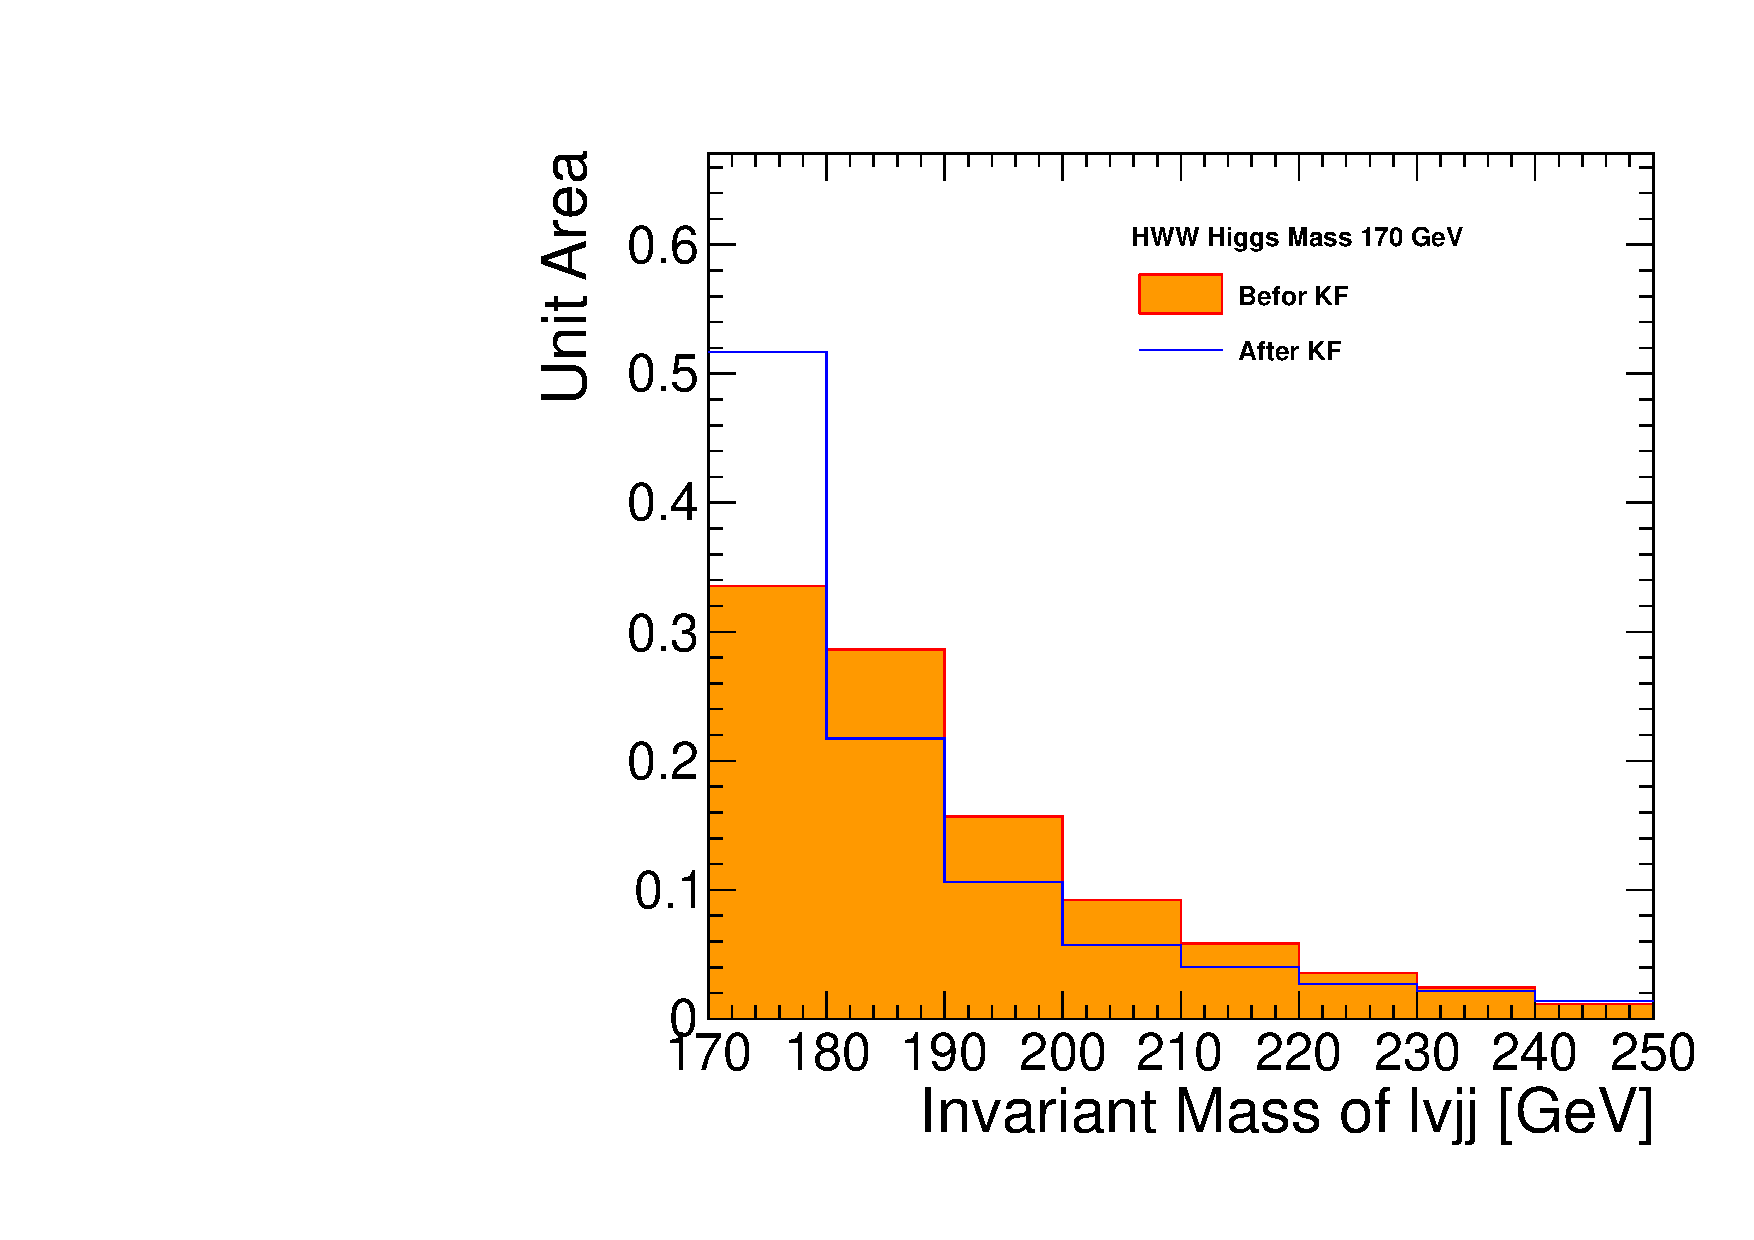
\includegraphics[width=0.42\textwidth]{plots/kfcompare-Hww170.pdf}
    }
    \subfigure[Higgs M=180~GeV]{
      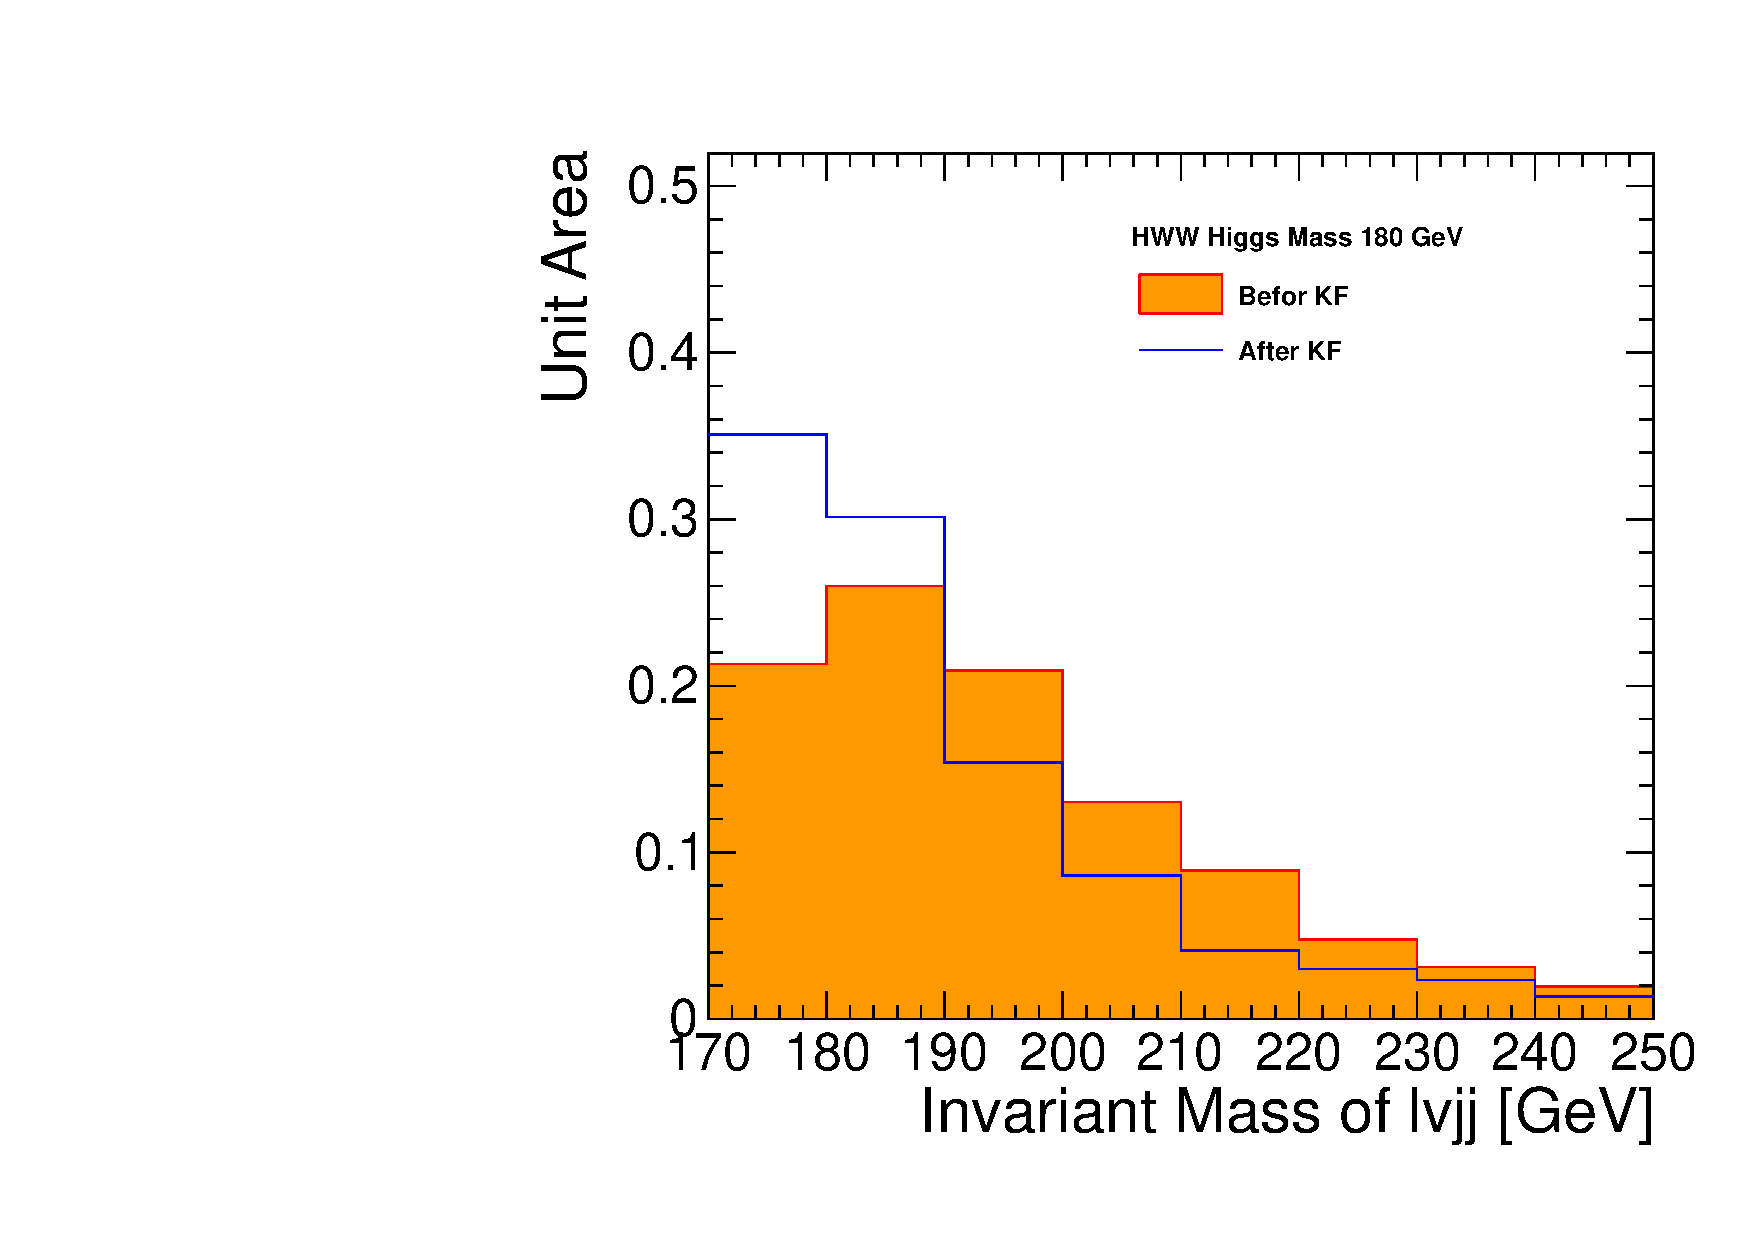
\includegraphics[width=0.42\textwidth]{plots/kfcompare-Hww180.pdf}
    }
    \\
    \subfigure[Higgs M=190~GeV]{
      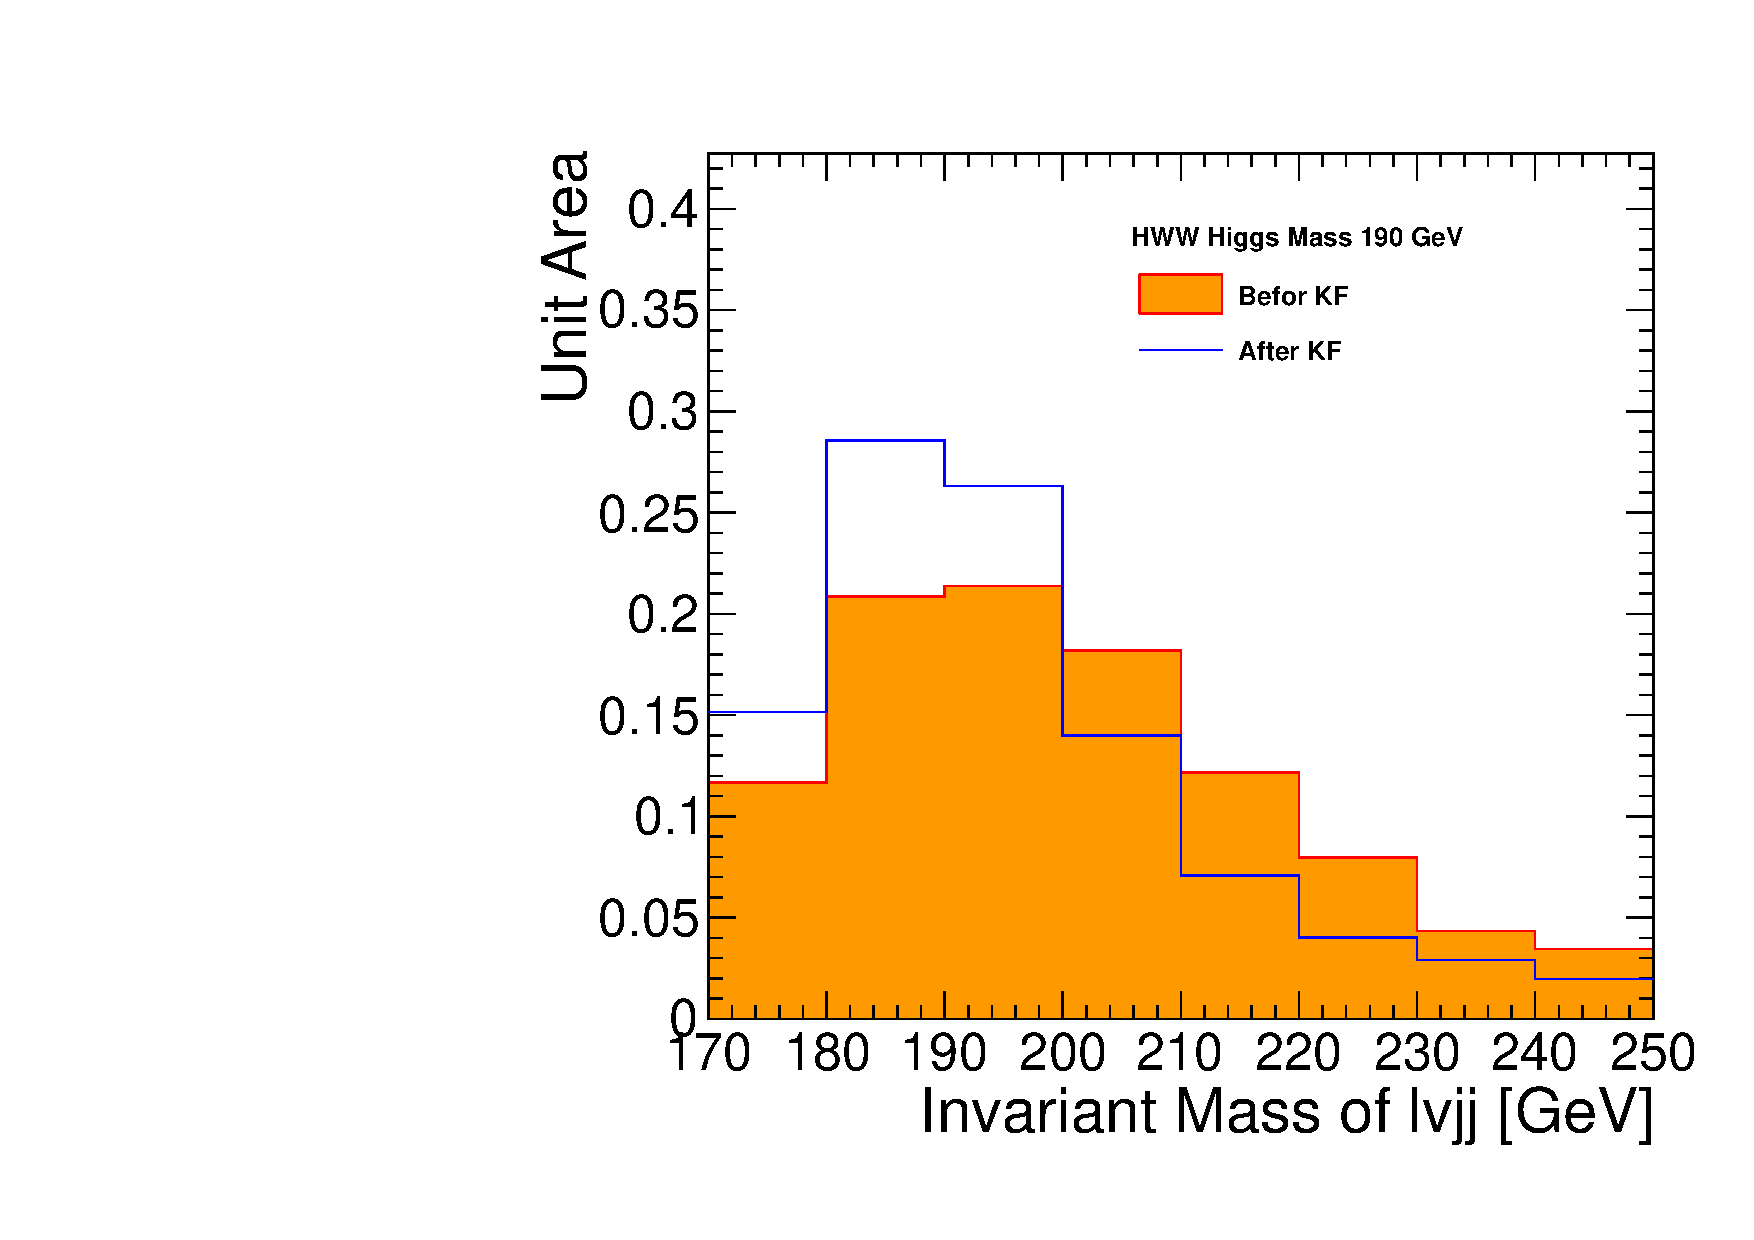
\includegraphics[width=0.42\textwidth]{plots/kfcompare-Hww190.pdf}
    }
    \subfigure[Higgs M=200~GeV]{
      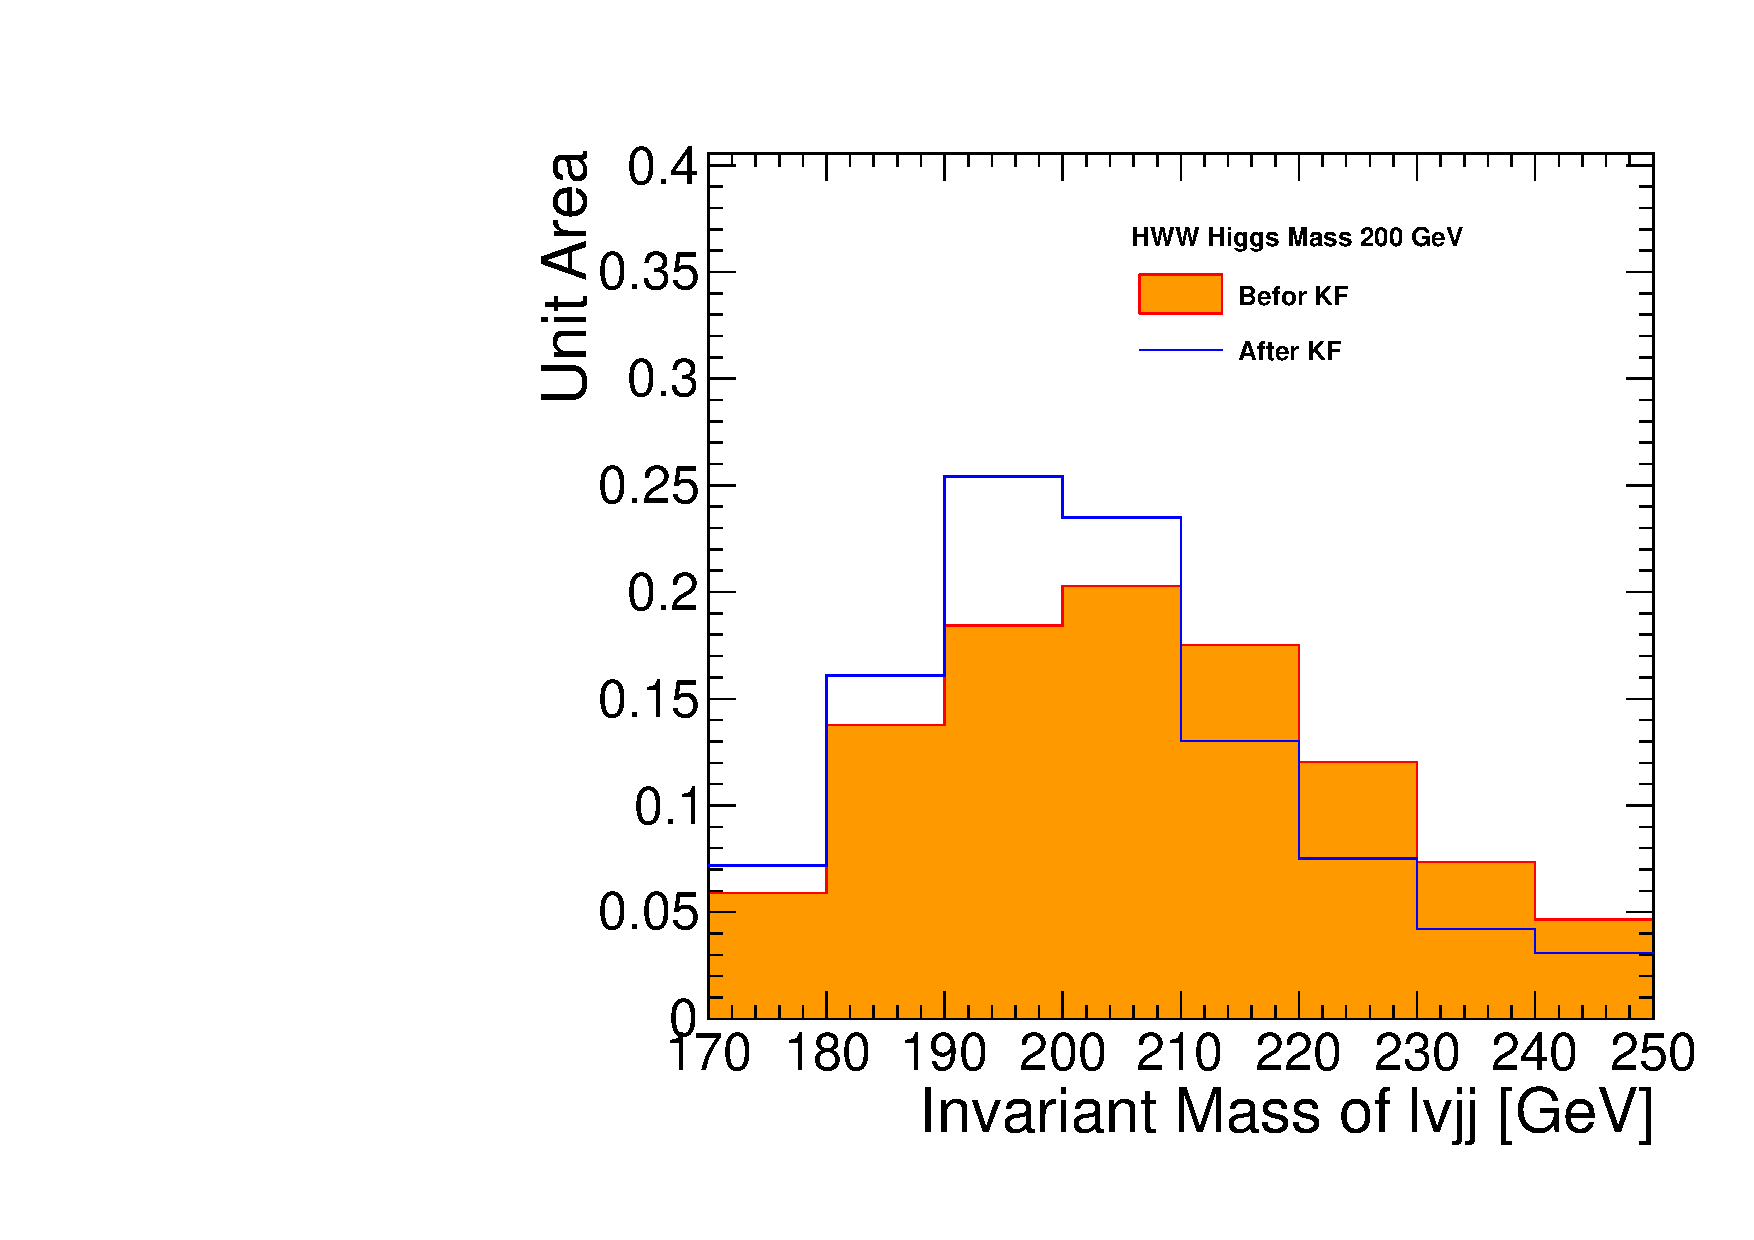
\includegraphics[width=0.42\textwidth]{plots/kfcompare-Hww200.pdf}
    }
    \\
    \subfigure[WW]{
      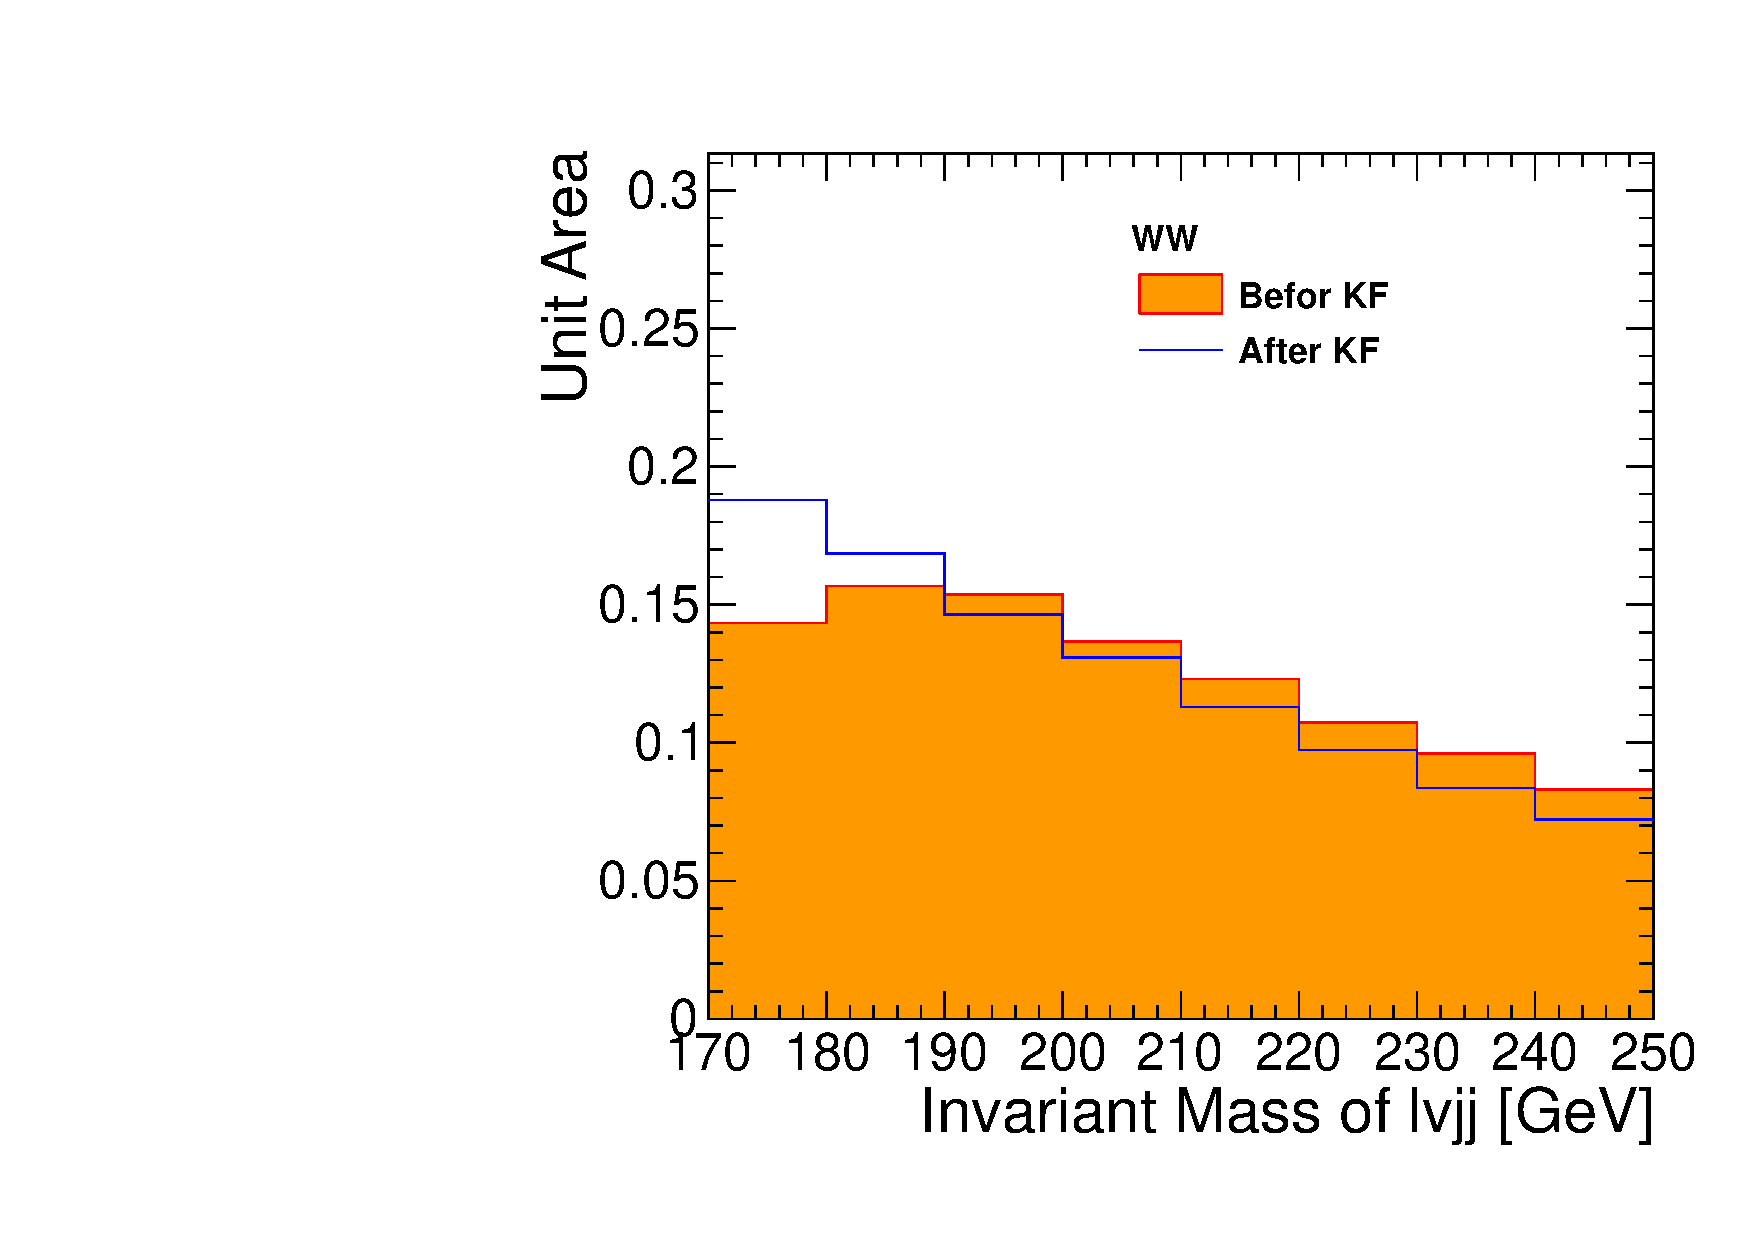
\includegraphics[width=0.42\textwidth]{plots/kfcompare-WW_low.pdf}
    }
    \subfigure[W+Jets]{
      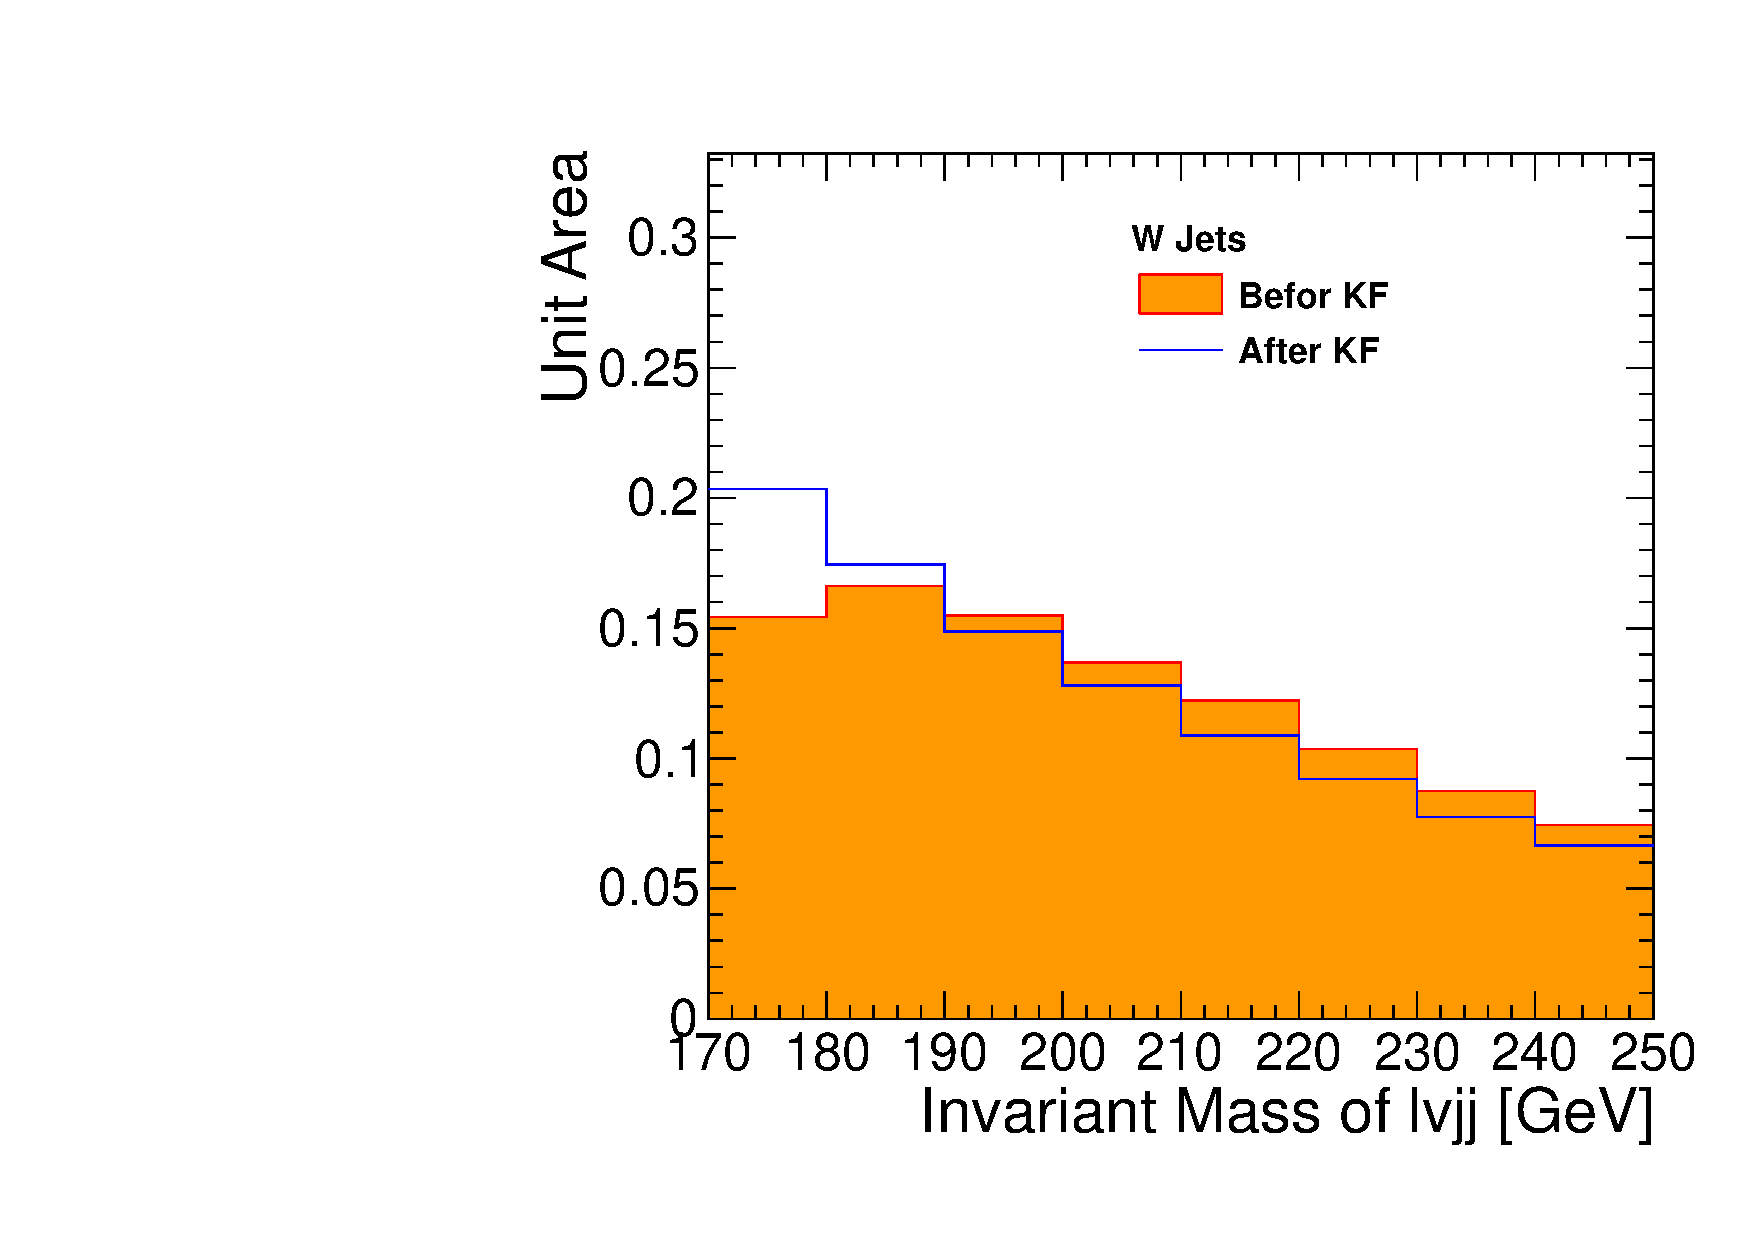
\includegraphics[width=0.42\textwidth]{plots/kfcompare-Wjet_low.pdf}
    }
    \caption{The four-body mass distributions obtained before and
             after the kinematic fit are reported for the four lowest
             Higgs mass hypotheses as well as for WW and W+Jets
             backgrounds. The mass range is constrained to that used
             for subsequent template modeling and limit setting.}
    \label{fig:fitKFExample}
\end{figure}
%
\clearpage
